% Convexification term over a relaxed one-hot variable (Fig. convexification).
\begin{tikzpicture}
  \begin{axis}[
      width=0.6\linewidth, height=0.42\linewidth,
      xmin=-0.05, xmax=1.05, ymin=-1.12, ymax=0.2,
      xtick={0,0.5,1}, ytick={-1,-0.5,-0.25,0},
      yticklabels={$-1$,$-\tfrac12$,$-\tfrac14$,$0$},
      xlabel={relaxed one-hot variable $\alpha_{j,k}$},
      ylabel={$\kappa\,\alpha_{j,k}(\alpha_{j,k}-1)$},
      axis lines=left, tick align=outside, clip=false,
      legend style={draw=none, fill=none, font=\footnotesize,
                    at={(1.04,0.5)}, anchor=west},
      legend cell align=left,
      every axis plot/.append style={thick, domain=0:1, samples=101},
    ]
    \draw[black!40, thin] (axis cs:-0.05,0) -- (axis cs:1.05,0);
    \addplot[black!35] {1*x*(x-1)};  \addlegendentry{$\kappa = 1$}
    \addplot[black!60, dashed] {2*x*(x-1)};  \addlegendentry{$\kappa = 2$}
    \addplot[black] {4*x*(x-1)};  \addlegendentry{$\kappa = 4$}
    \addplot[only marks, mark=*, mark size=2pt, black, forget plot]
      coordinates {(0,0) (1,0)};
    \addplot[only marks, mark=o, mark size=1.8pt, black, forget plot]
      coordinates {(0.5,-0.25) (0.5,-0.5) (0.5,-1)};
    \node[font=\footnotesize, anchor=south] at (axis cs:0.5,0.02)
      {zero at the integer values $0$ and $1$};
    \node[font=\footnotesize, anchor=west] at (axis cs:0.56,-0.97)
      {minimum $-\kappa/4$ at $\alpha_{j,k} = 1/2$};
  \end{axis}
\end{tikzpicture}
